\documentclass{thesis}
\usepackage{biblatex}
\usepackage{lipsum}
\usepackage{amssymb}
\usepackage{amsmath}
\usepackage{amsthm}
\usepackage{pdfpages}
\usepackage{graphicx}
\graphicspath{{Images/}}

\makeatletter
\def\@makechapterhead#1{%
  \vspace*{50\p@}%
  {\parindent \z@ \raggedright \normalfont
    \interlinepenalty\@M
    \Huge \bfseries #1\par\nobreak
    \vskip 40\p@
  }}
\def\@makeschapterhead#1{%
  \vspace*{50\p@}%
  {\parindent \z@ \raggedright
    \normalfont
    \interlinepenalty\@M
    \Huge \bfseries  #1\par\nobreak
    \vskip 40\p@
  }}
\makeatother

% Double spacing, if you want it.
% \def\dsp{\def\baselinestretch{2.0}\large\normalsize}
% \dsp

% If the Grad. Division insists that the first paragraph of a section
% be indented (like the others), then include this line:
% \usepackage{indentfirst}

\newtheorem{theorem}{Theorem}
\newtheorem{definition}{Definition}
\newtheorem{remark}{Remark}


\bibliography{references}



\begin{document}

% Declarations for Front Matter

\title{On the Birkhoff Conjecture for Convex Billiards}
\author{Han Yong Wunrow}
\degreesemester{Spring}
\degreeyear{2017}
\degree{Bachelor of Science}
\chair{Professor Richard Francis Sony}
\othermembers{Professor Roger Spam \\
  Associate Professor Michael Chex}
\numberofmembers{3}
\field{Mathematics: Genomics Specialization}
\campus{Twin Cities}
\date{\today}


% The title page generated by LaTeX is now acceptable for handing in.
% (This was not always the case).

\maketitle

% (This is included by thesis.tex; you do not latex it by itself.)

\begin{abstract}
The Birkhoff conjecture claims that if a convex billiard is integrable, then the boundary is necessarily an ellipse. In this paper, we analyze a local version of this conjecture that a small integrable perturbation of an ellipse must be an ellipse as proven in \cite{Kaloshin2016} by Kaloshin and Sorrentino. As an introduction, we discuss the behavior of billiards in a disc and in an ellipse. We then move onto some of the properties of a near-elliptical billiard. The dynamics of this system are modeled by a two-dimensional nonlinear mapping. The phase space of such billiards are of mixed kind with chaotic and regular behavior. We conclude by analyzing the behavior of the positive Lyapunov exponent and integrability of our system. 
\end{abstract}


\begin{frontmatter}

\tableofcontents
\clearpage
\listoffigures

\end{frontmatter}

\pagestyle{headings}

% (Optional) \part{First Part}

\chapter{Background}

Starting with the works of George David Birkhoff in early 1927, billiards have grown to become a popular topic of investigation in the framework of the theory of dynamical systems. Billiard systems are further remarkable for their appearance in a number of problems from optics, accoustics, and classical mechanics.

Similar to billiards in real life, the concept of a billiards system is fairly simple: you have a table and a ball, but in this case the ball has no mass so there is no friction. The ball hits the boundaries of the table and bounces off as it normally would. That is, it moves along in a straight line until it hits the edge of the table where it bounces off such that the angle of incidence equals the angle of reflection. Such systems become increasingly interesting in studying the trajectory of the ball as we change parameters such as the initial position, initial angle, and even the shape of the table. 

\begin{figure}[h]
    \centering
    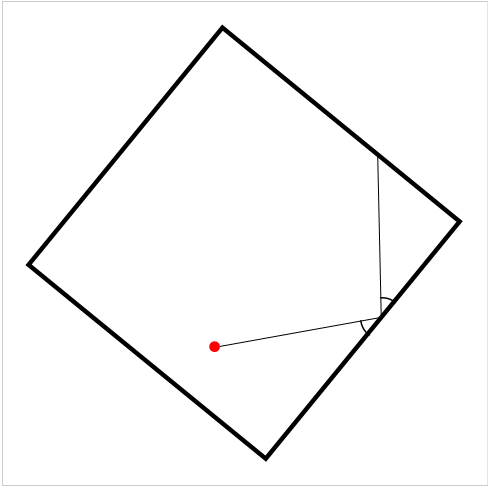
\includegraphics[scale = 0.45]{CongruentAngles}
    \caption{Square Billiard where angle of incidence equals the angle of reflection}
    \label{fig:my_label}
\end{figure}

\section{Billiard Map}
We can express these trajectories in the context of a dynamical system. Let $\theta \in [0,2\pi)$ be the angular position measured in radians from the $x$-axis and $\alpha \in (0, \pi)$ be the angle of reflection as shown in Figure \ref{billiardmap}.

\begin{figure}[h]
    \centering
    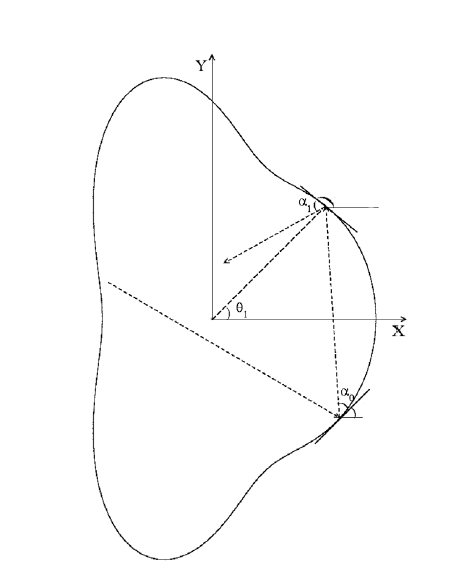
\includegraphics{BilliardMap}
    \caption{Illustration of particle's trajectory}
    \label{billiardmap}
\end{figure}
The billiard ball map for this discrete dynamical system is defined as follows
\begin{equation}
\begin{split}
    f: [0, 2\pi) \times (0,\pi) &\rightarrow [0, 2\pi) \times (0,\pi) \\
    (\theta_n,\alpha_n) &\mapsto (\theta_{n+1},\alpha_{n+1})
\end{split}
\end{equation}
There are two main restrictions on what shape our billiard can be. Let $\Omega \subset \mathbb{R}^2$ be a convex domain. We denote $\partial \Omega$ to be the boundary of the billiard. We require that the boundary of our billiard to be:
\begin{itemize}
    \item convex, and 
    \item smooth
\end{itemize}
Note that if the boundary is not convex, then $f$ is not continuous. This is because there may be trajectories that are tangent to the boundary on the inside. If such trajectories are perturbed slightly, the resulting trajectory is drastically changed. We require the boundary to be smooth since the motion of a trajectory that hits a corner is not well defined. Now that we have laid out the basics of the billiard dynamical system, we examine trajectories in a few elementary boundaries.

\section{Billiard in the Disc}
Although the billiard in a disc is one of the simplest billiards to analyze, there are a few interesting properties. Due to its geometry, the billiard map in a disc can be described by a very simple system of equations.
\begin{equation}
    \begin{pmatrix} \theta_{n+1} \\ \alpha_{n+1} \end{pmatrix} = \begin{pmatrix} 1 & 2 \\ 0 & 1 \end{pmatrix} \times \begin{pmatrix} \theta_n \\ \alpha_n \end{pmatrix}     
\end{equation}
The angle of reflection remains constant after each iteration, and the position angle along the boundary is obtained by rotating the previous position by $2\alpha$. 
An interesting remark is that if $\alpha_0$ is $\pi$-rational, then our orbit is periodic. Otherwise if $\alpha_0$ is $\pi$-irrational, then the orbit is dense and hits every position along our boundary. Orbits of both types along with their phase space diagrams can be seen in figures \ref{disc1} and \ref{disc2}.

\begin{figure}[h]
    \centering
    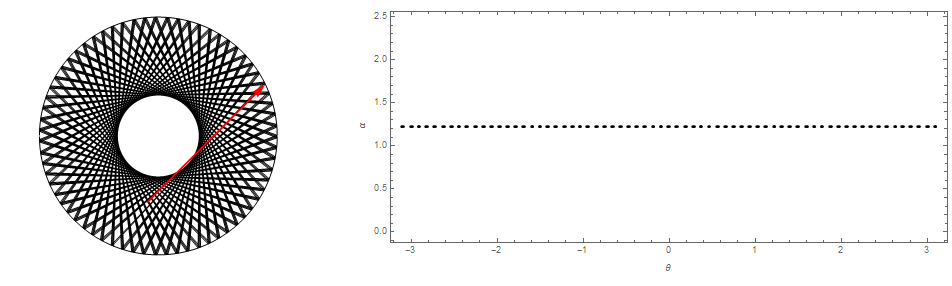
\includegraphics[scale = 0.8]{DiscPhaseSpace1}
    \caption{Disc Billiard with dense orbit}
    \label{disc1}
\end{figure}
\begin{figure}[h]
    \centering
    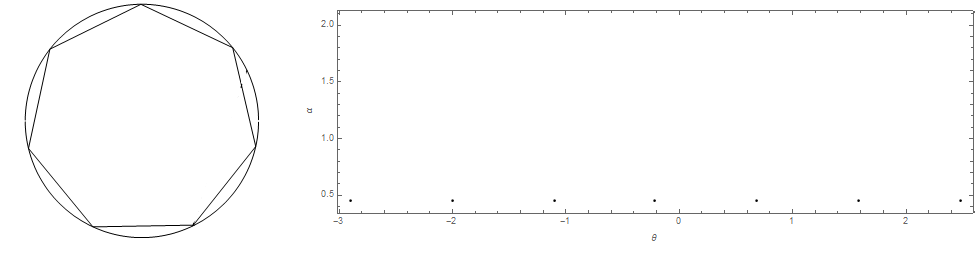
\includegraphics[scale = 0.8]{DiscPhaseSpace2}
    \caption{Disc Billiard with periodic orbit}
    \label{disc2}
\end{figure}
One should take note of the concentric circle that is formed by the trajectories that stay tangent to it in Figure \ref{disc1}. We refer to such curves as caustics. 
\begin{definition}
A curve $\Gamma \subset \Omega$ is said to be \textbf{caustic} if any billiard orbit having one segment tangent to $\Gamma$ has all its segments tangent to $\Gamma$.
\end{definition}
One should also take note of the formation of invariant curves in the phase space corresponding to particular caustics. These relationships will be examined further in the next section. 

\section{Billiard in the Ellipse}
We now consider billiards in slightly more complex shapes - ellipses where the boundary $\partial \Omega$ is defined by 
\begin{equation}
    \frac{x^2}{a} + \frac{y^2}{b} = 1 \text{   where } a > b
\end{equation}
The trajectory in an elliptical billiard is related to its \textit{confocal} conic sections. We say two conic sections are \textit{confocal} if they share the same foci. 
\begin{remark}
\label{caustic}
A billiard trajectory inside $\Omega$ stays tangent to a caustic fixed confocal ellipse or hyperbola. More precisely, the billiard trajectories in $\Omega$ stay tangent to a caustic 
\begin{equation}
    \mathbb{C}_{\lambda} \in \Big \{\frac{x^2}{a - \lambda} + \frac{y^2}{b - \lambda} = 1 \Big \}
\end{equation}
where $a > b$.
\end{remark}

\begin{proof}
This result is equivalent to Poncelet's closure theorem and its elementary geometric proof is shown in \cite{Tabachnikov2011}.
\end{proof}

It is necessarily true that the confocal conics of $\Omega$ are either hyperbolas or ellipses. Consider the function
\begin{equation}
    \label{f}
    f = \frac{x^2}{a - \lambda} + \frac{y^2}{b - \lambda} - 1 = 0 \hspace{10mm} a > b
\end{equation}
For fixed values of $x$ and $y$ we can graph $f$ as a function of $\lambda$ as shown in figure \ref{ConfocalGraph}. 
\begin{figure}[h]
    \centering
    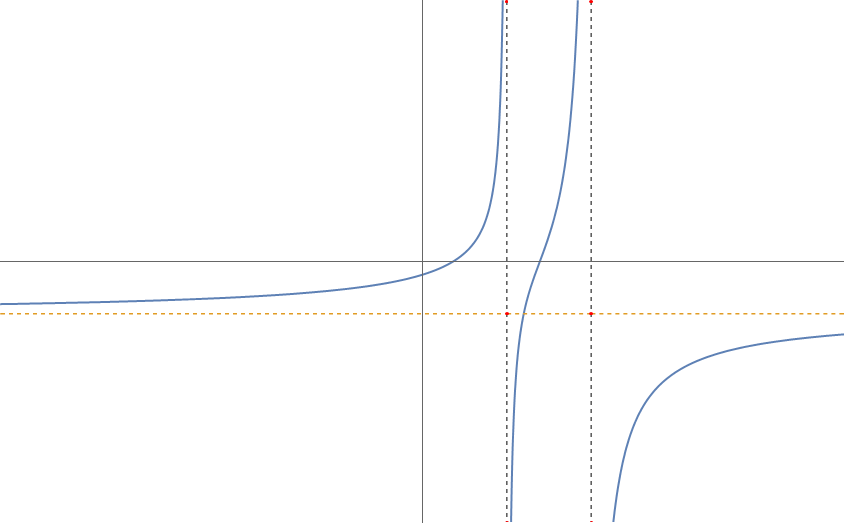
\includegraphics[scale = 0.35]{ConfocalGraph}
    \caption{Graph of $f$ as a function of $\lambda$ for fixed $x$ and $y$}
    \label{ConfocalGraph}
\end{figure}
As seen in the graph the roots are $\lambda_1 \in (-\infty, b)$ and  $\lambda_2 \in (b,a)$. Note that $\lambda = 0$ defines the original ellipse $\partial \Omega$ and since we are only interested in confocal conics contained within $\partial \Omega$, $\lambda_1 \in (0, b)$. For $\lambda = \lambda_1$ equation \ref{f} defines an ellipse, and for $\lambda = \lambda_2$ it defines a hyperbola. Trajectories of both types are shown below in figures \ref{ConfocalEllipse} and \ref{ConfocalHyperbola}.
\newpage
\begin{figure}[h]
    \centering
    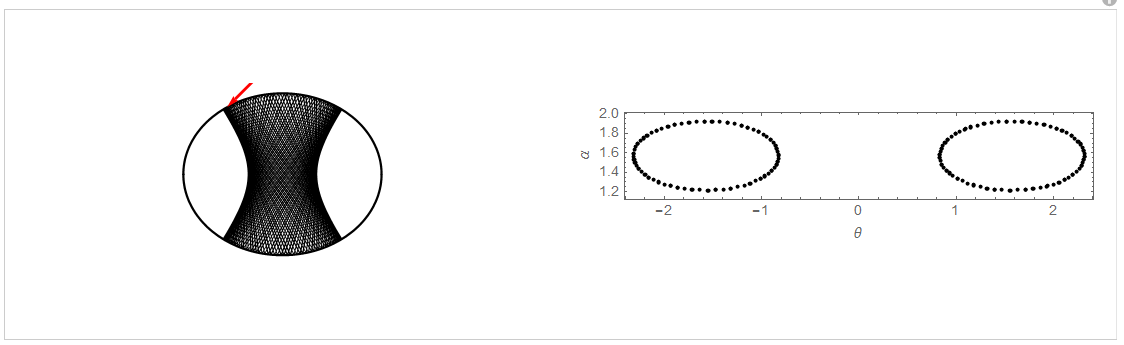
\includegraphics[width = 1\textwidth]{EllipsePhaseSpace3}
    \caption{Confocal Hyperbola Elliptical Billiard with Phase Space Diagram $a = 1, b = 1.5$}
    \label{ConfocalHyperbola}
\end{figure}
\begin{figure}[h]
    \centering
    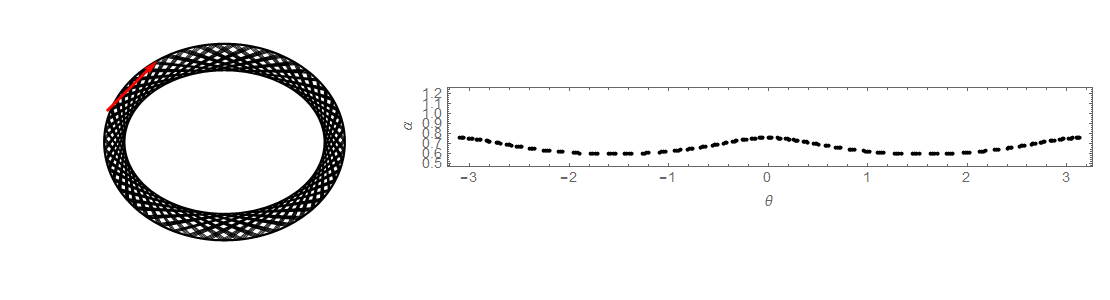
\includegraphics[width = 0.9\textwidth]{EllipsePhaseSpace}
    \caption{Confocal Ellipse Elliptical Billiard with Phase Space Diagram $a = 1, b = 1.5$}
    \label{ConfocalEllipse}
\end{figure}
\begin{figure}[h]
    \centering
    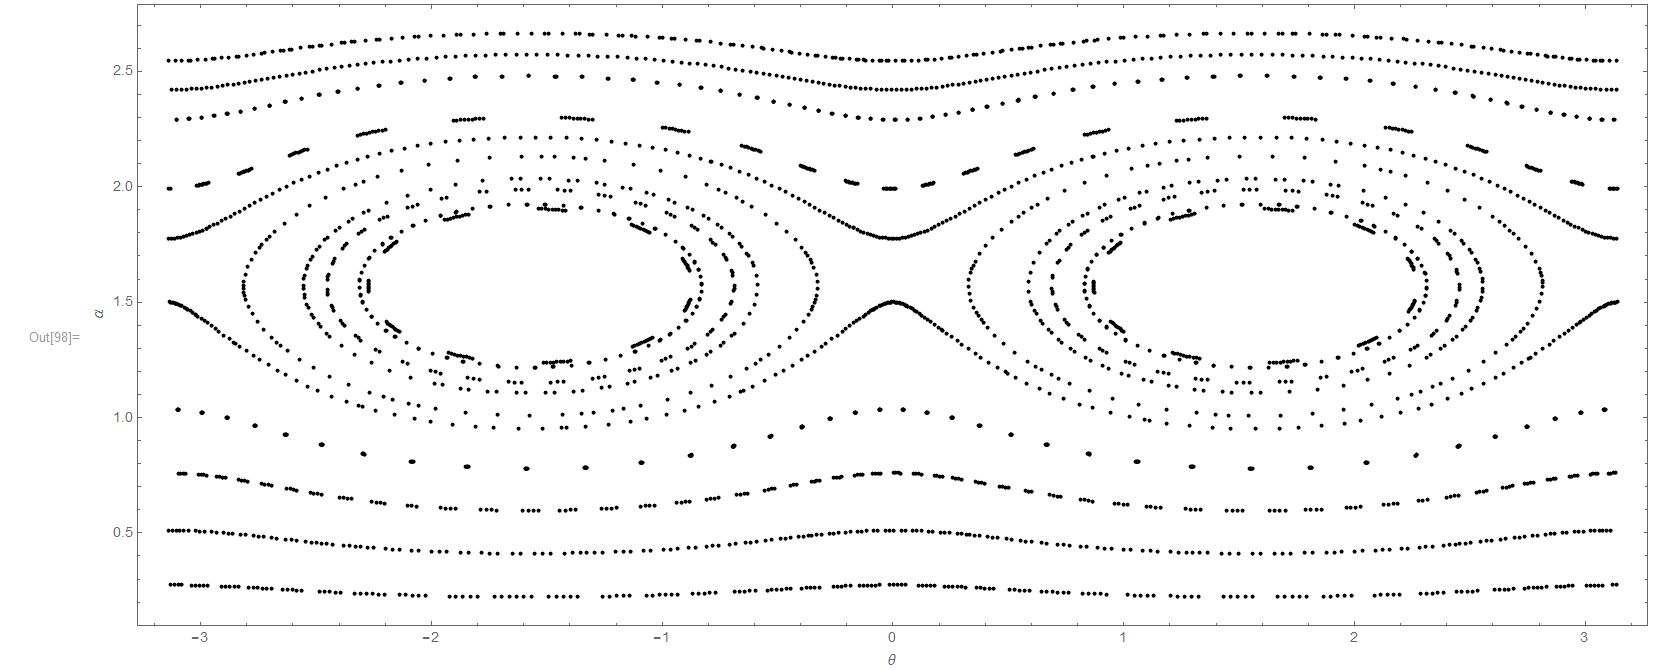
\includegraphics[scale = 0.39]{EllipsePhaseSpace2}
    \caption{Elliptical Billiard Phase Space Diagram $a = 1, b = 1.5$}
    \label{EllipsePS}
\end{figure}
Similarly to a billiard in a disc, one can see a relationship between invariant curves in the phase space that correspond to either a confocal hyperbola or confocal ellipse caustic.    If we plot these invariant curves for multiple initial conditions as seen in Figure \ref{EllipsePS}, one can see that the phase space is completely foliated by invariant curves of the billiard map $f$. 

This brings us to the topic of \textit{integrability}. A billiard in an ellipse (and also a disc) are examples of \textit{integrable billiards}. 
\begin{definition}
A billiard is said to be \textbf{integrable} if there exists a (smooth) foliation of the whole phase space consisting of invariant curves of the billiard map
\end{definition}
\newpage

\begin{remark}
A billiard in an ellipse is integrable.
\end{remark}

\begin{proof}
All the trajectories tangent to a elliptic caustic lie on a curve in the manifold $M$ that is invariant under $f$. Those invariant curves appear as deformations of the invariant lines $\alpha = c$ for some constant $c$ as in the circular billiard. All the trajectories tangent to a hyperbolic caustic lie on two closed curves in $M$. Each curve is invariant under $f^2$. Therefore, the surface $M$ is completely foliated by invariant curves and thus elliptical billiards are integrable. 
\end{proof}

It is well known that elliptical billiards are integrable. However, a long standing open problem in billiard systems is the converse. That is, proving that the only integrable billiards are ellipses.

\section{Birkhoff Conjecture}

\textbf{Birkhoff Conjecture} \textit{If a billiard in }$\Omega$ \textit{ is integrable}, \textit{then the boundary } $\partial\Omega$ \textit{ is an ellipse.}
\newline

Birkhoff's question of the existence of other integrable billiards other than ellipses has long been studied. We will briefly describe the progress that has been made to towards proving this conjecture.
In \cite{Mather1982}, Mather proved the non-existence of caustics (hence, the non-integrability) if the curvature of the boundary vanishes at one point. This further justifies our restriction to strictly convex billiards. As stated by Mather,

We will say a trajectory is $\varepsilon$-glancing if for at least one bounce the angle of reflection (with either the positive or negative tangent of $\partial \Omega$ at the point of reflection) is $ < \varepsilon$. If  $\varepsilon < \pi/2$ , we can distinguish between a positively  $\varepsilon$-glancing trajectory and
a negatively $\varepsilon$-glancing trajectory according to whether it is the positive or negative tangent to $\partial \Omega$ which the direction of reflection is close to.
A trajectory might be positively $ \varepsilon$-glancing at one bounce and negatively $\varepsilon$-glancing at another bounce. Thus, one can ask whether for every  $\varepsilon> 0$, there exist
trajectories which are both positively and negatively $\varepsilon$ -glancing. We will prove a
theorem which shows in some cases the answer is yes.
\begin{theorem}
If the curvature of $\partial \Omega$ vanishes at some point, then for every  $\varepsilon > 0$, there exist trajectories which are both positively and negatively  $\varepsilon$-glancing. (Mather; 1982)
\end{theorem}

In \cite{Bialy1993}, Bialy proved the following result concerning global integrability.

\begin{theorem}
 If the phase space of the billiard ball map is globally foliated by continuous invariant curves which are not null-homotopic, then it is the circular billiard. (Bialy; 1993)
\end{theorem}

More recently, in \cite{Avila2016}, Avila, De Simoi, and Kaloshin proved a local version of this conjecture for ellipses with small eccentricity.

\begin{theorem}
A small integrable perturbation of an ellipse of small eccentricity must be an ellipse. (Avila, Simoi, Kaloshin; 2016)
\end{theorem}

In \cite{Kaloshin2016}, Kaloshin and Sorrentino expand upon this result in which they prove a local version of this conjecture for arbitrary eccentricity.

\begin{theorem}
 A small integrable perturbation of an ellipse of arbitrary eccentricity must be an ellipse. (Kaloshin, Sorrentino; 2017)
\end{theorem}

Note that Theorems 3 and 4 are only local versions of this conjecture. That is, there still may be examples of integrable billiards that are very different from ellipses. In the following section, similarly to in \cite{Kaloshin2016}, we will analyze the integrability of perturbations of elliptical billiards with arbitrary eccentricity.
\chapter{Near Elliptical Billiard}

\section{Billiard Mapping}

We define the boundary of a near elliptical billiard to be
\[
    a x^2 + b y^2 + \varepsilon x^4 = 1.
\]
We begin by discussing the details needed for the construction of the billiard map that describes the dynamics of this problem. The radius of the boundary expressed in polar coordinates is given by
\begin{align}
          1 &=  R^2(a\cos^2\theta + b\sin^2\theta)  + R^4(\varepsilon\cos^4\theta) \\
          0 &= -1 + x(a\cos^2\theta + b\sin^2\theta)  + x^2(\varepsilon\cos^4\theta) \hspace{10mm} (x = R^2) \\
            R^2 = x &= \frac{-(a\cos^2\theta + b\sin^2\theta) \pm \sqrt{(a\cos^2\theta + b\sin^2\theta)^2 + 4(\varepsilon\cos^4\theta)}}{2(\varepsilon\cos^4\theta)} \\
R(\theta,a,b,\varepsilon) &= \sqrt{\frac{-(a\cos^2\theta + b\sin^2\theta) \pm \sqrt{(a\cos^2\theta + b\sin^2\theta)^2 + 4(\varepsilon\cos^4\theta)}}{2(\varepsilon\cos^4\theta)} } .
\end{align}
Given an initial position and direction $(\theta_n,\alpha_n)$, the angle between the vector tangent to the curve and the vector perpendicular to the reflected trajectory is given as
\begin{equation}
    \phi_n = \arctan\Big(\frac{Y'(\theta_n)}{X'(\theta_n)}\Big)
\end{equation}
where 
\begin{equation}
    X(\theta_n) = R(\theta_n)\cos(\theta_n)
\end{equation}
\begin{equation}
    Y(\theta_n) = R(\theta_n)\sin(\theta_n)
\end{equation}
and their derivatives are
\begin{equation}
    X'(\theta_n) = R'(\theta_n)\cos(\theta_n) - R(\theta_n)\sin(\theta_n) 
\end{equation}
and
\begin{equation}
    Y'(\theta_n) = R'(\theta_n)\sin(\theta_n) + R(\theta_n)\cos(\theta_n).
\end{equation}
To obtain the new position $\theta_{n+1}$ we must solve the equation
\begin{equation}
    Y(\theta_{n+1}) - Y(\theta_n) = \tan(\alpha_n + \phi_n)(X(\theta_{n+1}) - X(\theta_n))
\end{equation}
As seen in figure \ref{billiardmap} the next trajectory angle $\alpha_{n+1}$ is given by
\begin{equation}
    \alpha_{n+1} = \phi_{n+1} - (\alpha_n + \phi_n)
\end{equation}
Thus the billiard mapping is defined as
\begin{equation}
    \begin{cases} 
      F(\theta_{n+1}) = 0 = Y(\theta_{n+1}) - Y(\theta_n) - \tan(\alpha_n + \phi_n)(X(\theta_{n+1}) - X(\theta_n)) \\
      \alpha_{n+1} = \phi_{n+1} - (\alpha_n + \phi_n)
   \end{cases}
   \label{bmap}
\end{equation}

\section{Numerical Results}
Let us now discuss some of our results. Figures \ref{nearellipse1}, \ref{nearellipse2}, and \ref{nearellipse3} illustrate the destruction of both the confocal caustic and invariant curve in the phase space as we increase the parameter $\varepsilon$. As shown in Figures \ref{nearellipse4} and \ref{nearellipse5} we can see a complex hierarchy of behaviours in the phase space along with the formation of a large chaotic sea as we increase $\varepsilon$. 
\begin{figure}[h]
    \centering
    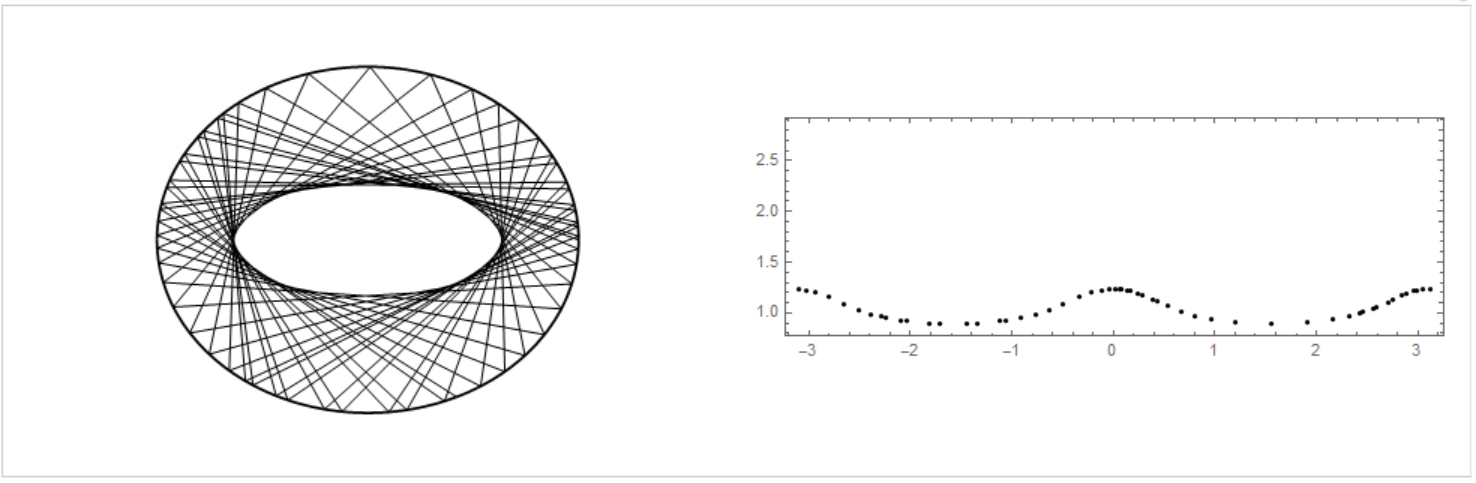
\includegraphics[width = 0.9\textwidth]{NearellipsePhaseSpace2}
    \caption{Near elliptical Billiard $a=1, b=1.5, \varepsilon = .01$ with Phase Space Diagram}
    \label{nearellipse1}
\end{figure}
\begin{figure}[h]
    \centering
    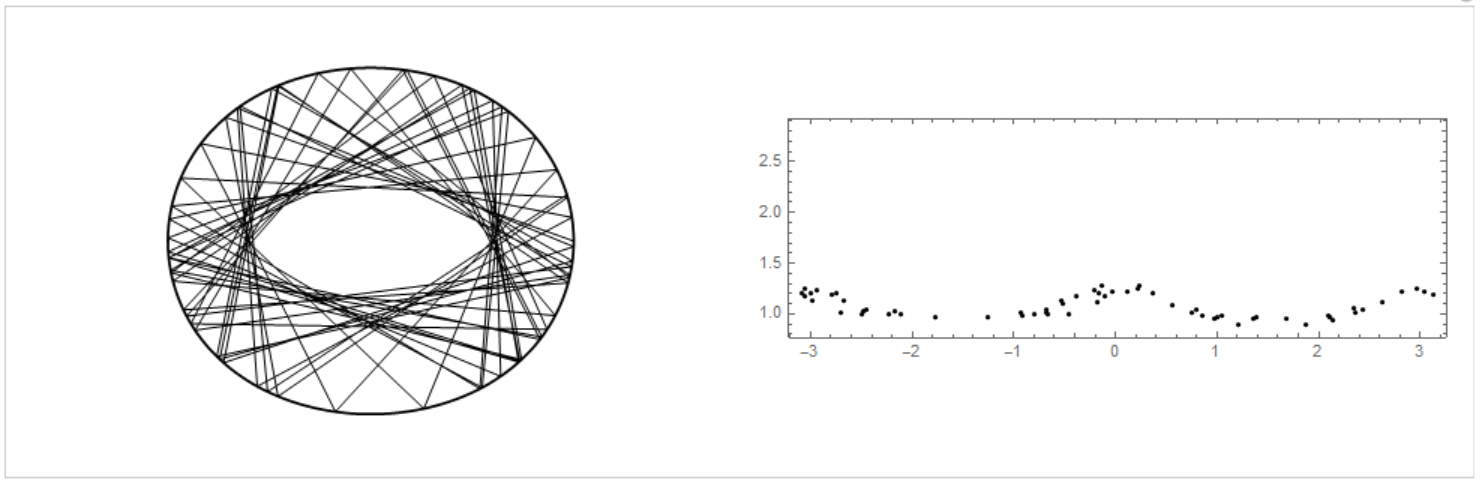
\includegraphics[width = 0.8\textwidth]{NearellipsePhaseSpace3}
    \caption{Near elliptical Billiard $a=1, b=1.5, \varepsilon = .1$ with Phase Space Diagram}
    \label{nearellipse2}
\end{figure}
\begin{figure}[h]
    \centering
    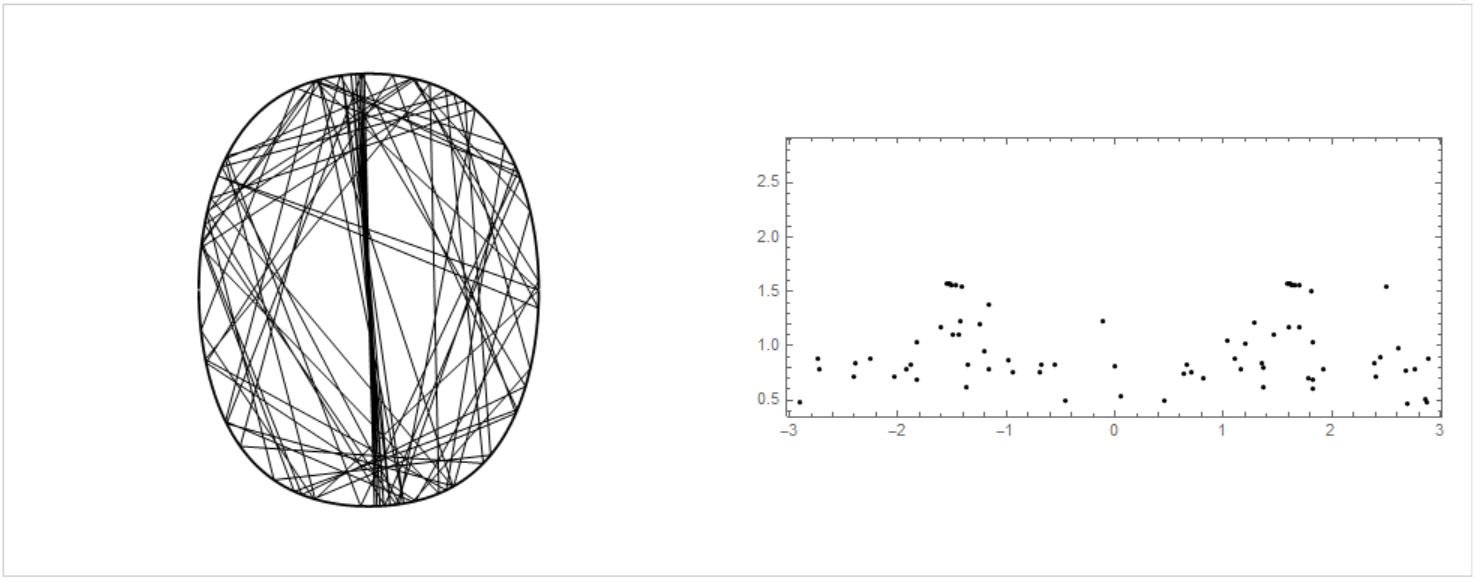
\includegraphics[width = 0.8\textwidth]{NearellipsePhaseSpace}
    \caption{Near elliptical Billiard $a=b=\varepsilon = 1$ with Phase Space Diagram}
    \label{nearellipse3}
\end{figure}

\begin{figure}[h]
    \centering
    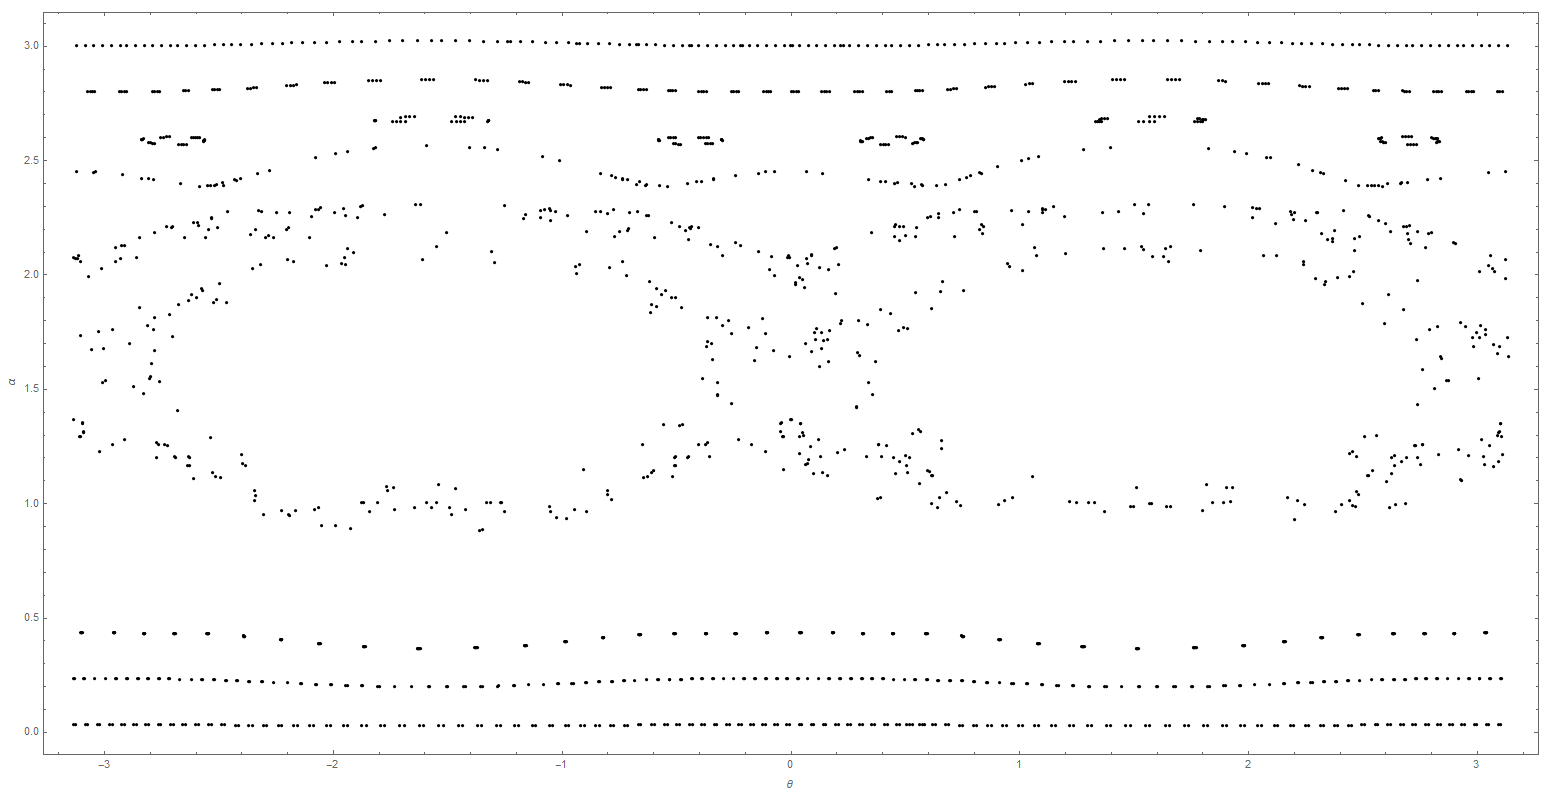
\includegraphics[width = 0.9\textwidth]{NearellipsePhaseSpace4}
    \caption{Near elliptical Billiard $a=1, b=1.5, \varepsilon = .1$ with Phase Space Diagram}
    \label{nearellipse4}
\end{figure}
\begin{figure}[h]
    \centering
    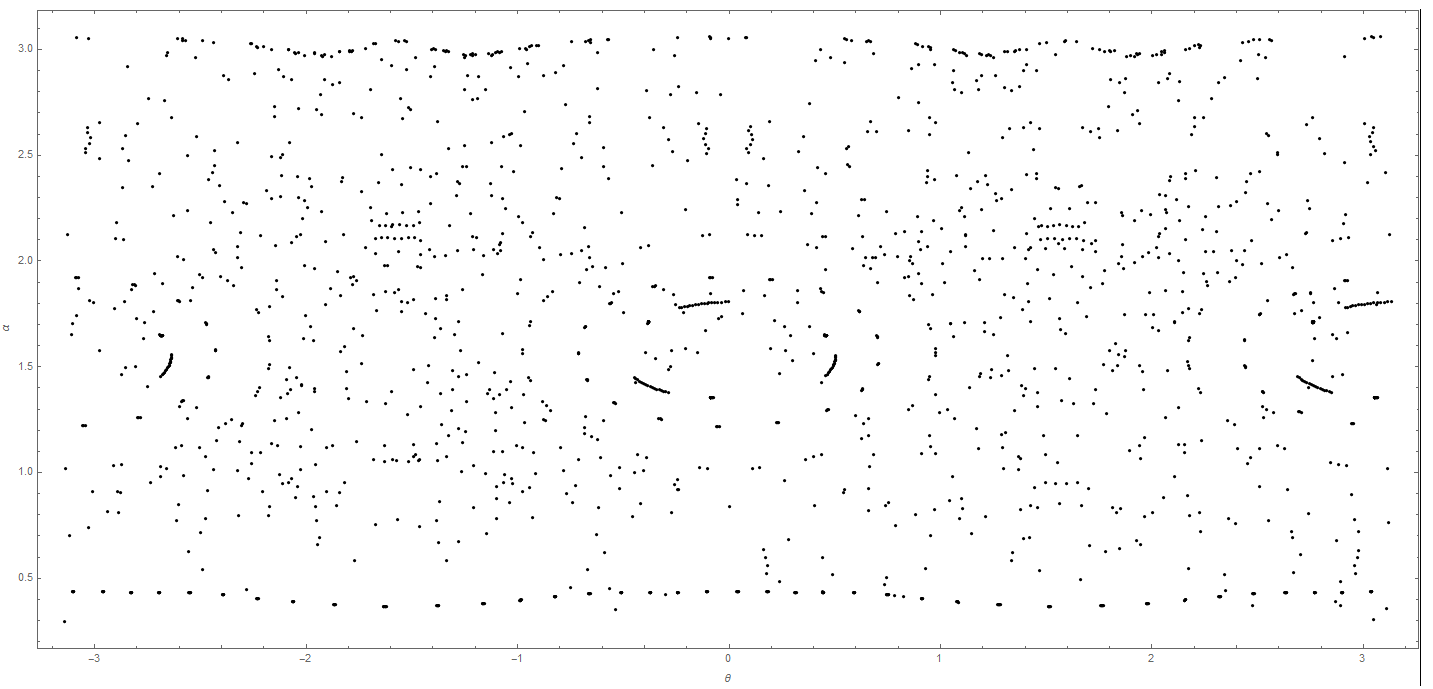
\includegraphics[width = 0.9\textwidth]{NearellipsePhaseSpace5}
    \caption{Near elliptical Billiard $a=1, b=1.5, \varepsilon = 10$ with Phase Space Diagram}
    \label{nearellipse5}
\end{figure}
Qualitatively, it is simple to see from the phase space diagrams that as we perturb an ellipse by increasing $\varepsilon$, the billiard no longer is integrable. To obtain a more quantitative sense of this chaotic motion we examine the Lyapunov exponent.
\begin{definition}
As discussed in \cite{Oliveira2010}, the \textbf{Lyapunov exponent} is defined as
\[
    \lambda_j = \lim_{n \rightarrow \infty} n^{-1} \log |\Lambda_j| \hspace{10mm} j = 1,2
\]
where $\Lambda_j$ are the eigenvalues of $M = \prod_{i = 1}^n J_i(\theta_i, \alpha_i)$ and $J_i$ is the Jacobian matrix evaluated over the orbit $(\theta_i, \alpha_i)$.
\end{definition}
It is well known that the Lyapunov exponent serves as a practical tool for studying the behavior of a dynamical system, and consequently whether the given system is chaotic. If the Lyapunov exponent converges to a positive value after significantly large $n$ we say that our system is chaotic. 
\newpage
Since our billiard mapping \ref{bmap} is not well defined to compute the product of Jacobians, we discuss a method to compute the Lyapunov exponents numerically. 
\begin{enumerate}
    \item Starting with initial conditions $\theta_{u0}$ and $\alpha_{u0}$ (call orbit $u$), choose a nearby point $(\theta_{v0}, \alpha_{v0})$ (call orbit $v$) that is within distance $d_0$.
    \item
    Iterate both orbits once and calculate the new distance $d_1$.
    \item
    Evaluate $\ln(d_1/d_0)$.
    \item
    Readjust the point along orbit $v$ so that its distance from the new point on orbit $u$ is $d_0$ and in the same direction as $d_1$. i.e.
    \[
        \theta_{v0} = \theta_{u1} + d_0(\theta_{v1} - \theta_{u1}) / d_1
    \] and
    \[
        \alpha_{v0} = \alpha_{u1} + d_0(\alpha_{v1} - \alpha_{u1}) / d_1
    \]
    \item Repeat steps 2 - 4 $n$ times and calculate a running average of step 3. 
\end{enumerate}
This process is illustrated in Figure \ref{dia}. 

\begin{figure}
    \centering
    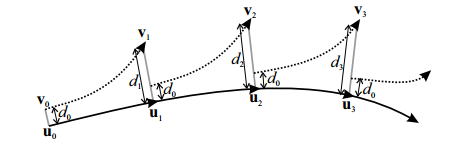
\includegraphics{diagram}
    \caption{Diagram of how to compute the Lyapunov Exponent numerically}
    \label{dia}
\end{figure}
Due to the precision of floating point numbers in Mathematica, we choose $d_0 = 10^{-8}$. To illustrate that our near elliptical billiard has a chaotic component in the phase space, we show in Figures \ref{lyap1} and \ref{lyap2} the behavior of the positive Lyapunov exponent as a function of the number of collisions $n$ for various initial conditions chosen in the chaotic sea. Each initial condition was iterated up to $500$ times. 
\begin{figure}
    \centering
    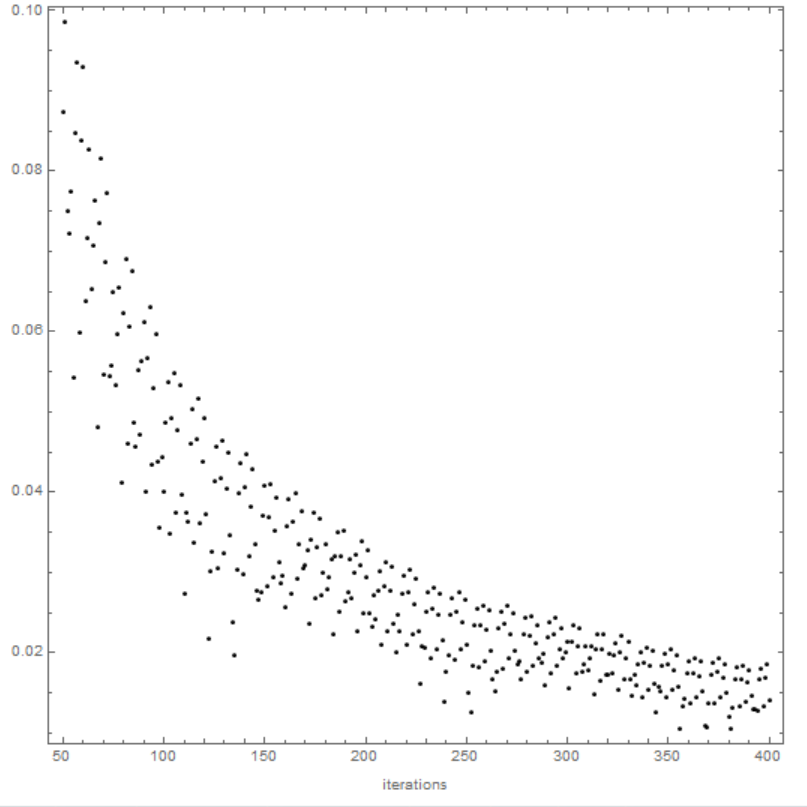
\includegraphics{lyap1}
    \caption{Behavior of the Lyapunov Exponent for $a = 1$, $b = 1.4$, and $\varepsilon$ = 1.5}
    \label{lyap1}
\end{figure}
\begin{figure}
    \centering
    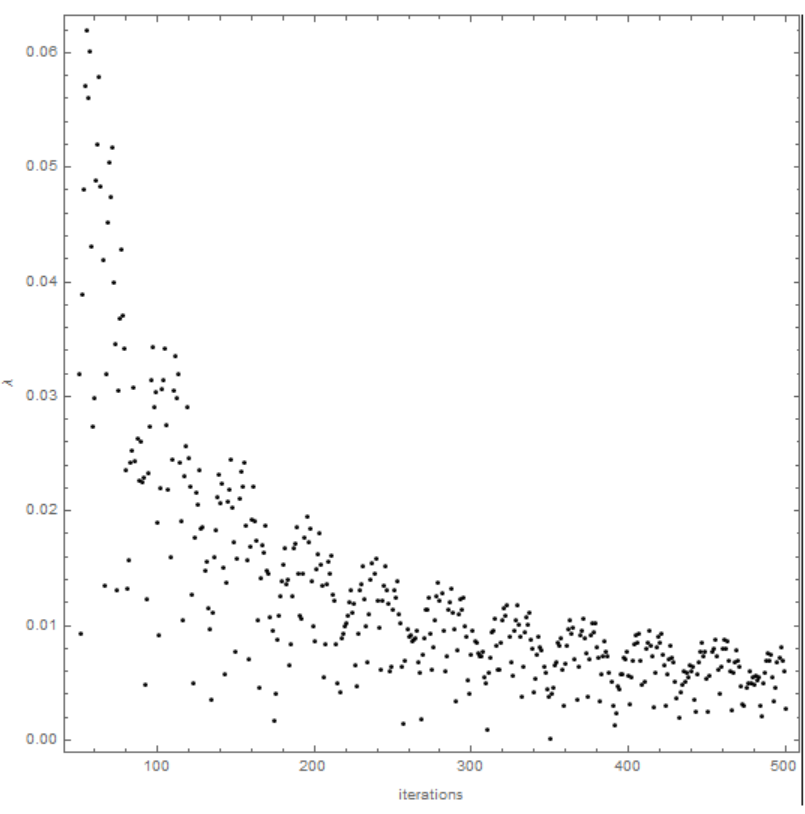
\includegraphics{lyap2}
    \caption{Behavior of the Lyapunov Exponent for $a = 1$, $b = 1.4$, and $\varepsilon$ = 0.1}
    \label{lyap2}
\end{figure}

In future work, many more iterations are needed to provide a proper convergence plot of the positive Lyapunov exponent. However, it is still clear to see from the plots that it will eventually converge to a positive value. As such we can conclude that the regions of our phase space for near elliptical billiards are chaoitic and that the system is no longer integrable due to the destruction of the invariant spanning curves in the phase space. 
\chapter{Conclusion}
As a conclusion, we have provided a brief background of the behavior of billiards in a disc and ellipse. We then obtained a nonlinear mapping that describe the dynamics of a near elliptical billiard. We have shown that the phase space has a mixed form, and lastly, we have shown that the Lyapunov exponent converges to a positive value and thus proves that near elliptical billiards are not integrable due to the destruction of some of the invariant spanning curves in the phase space. 
\chapter{Appendix}
We provide the Mathematica used to create the plots of trajectories in the paper along with the computations of the Lyapunov exponent. 
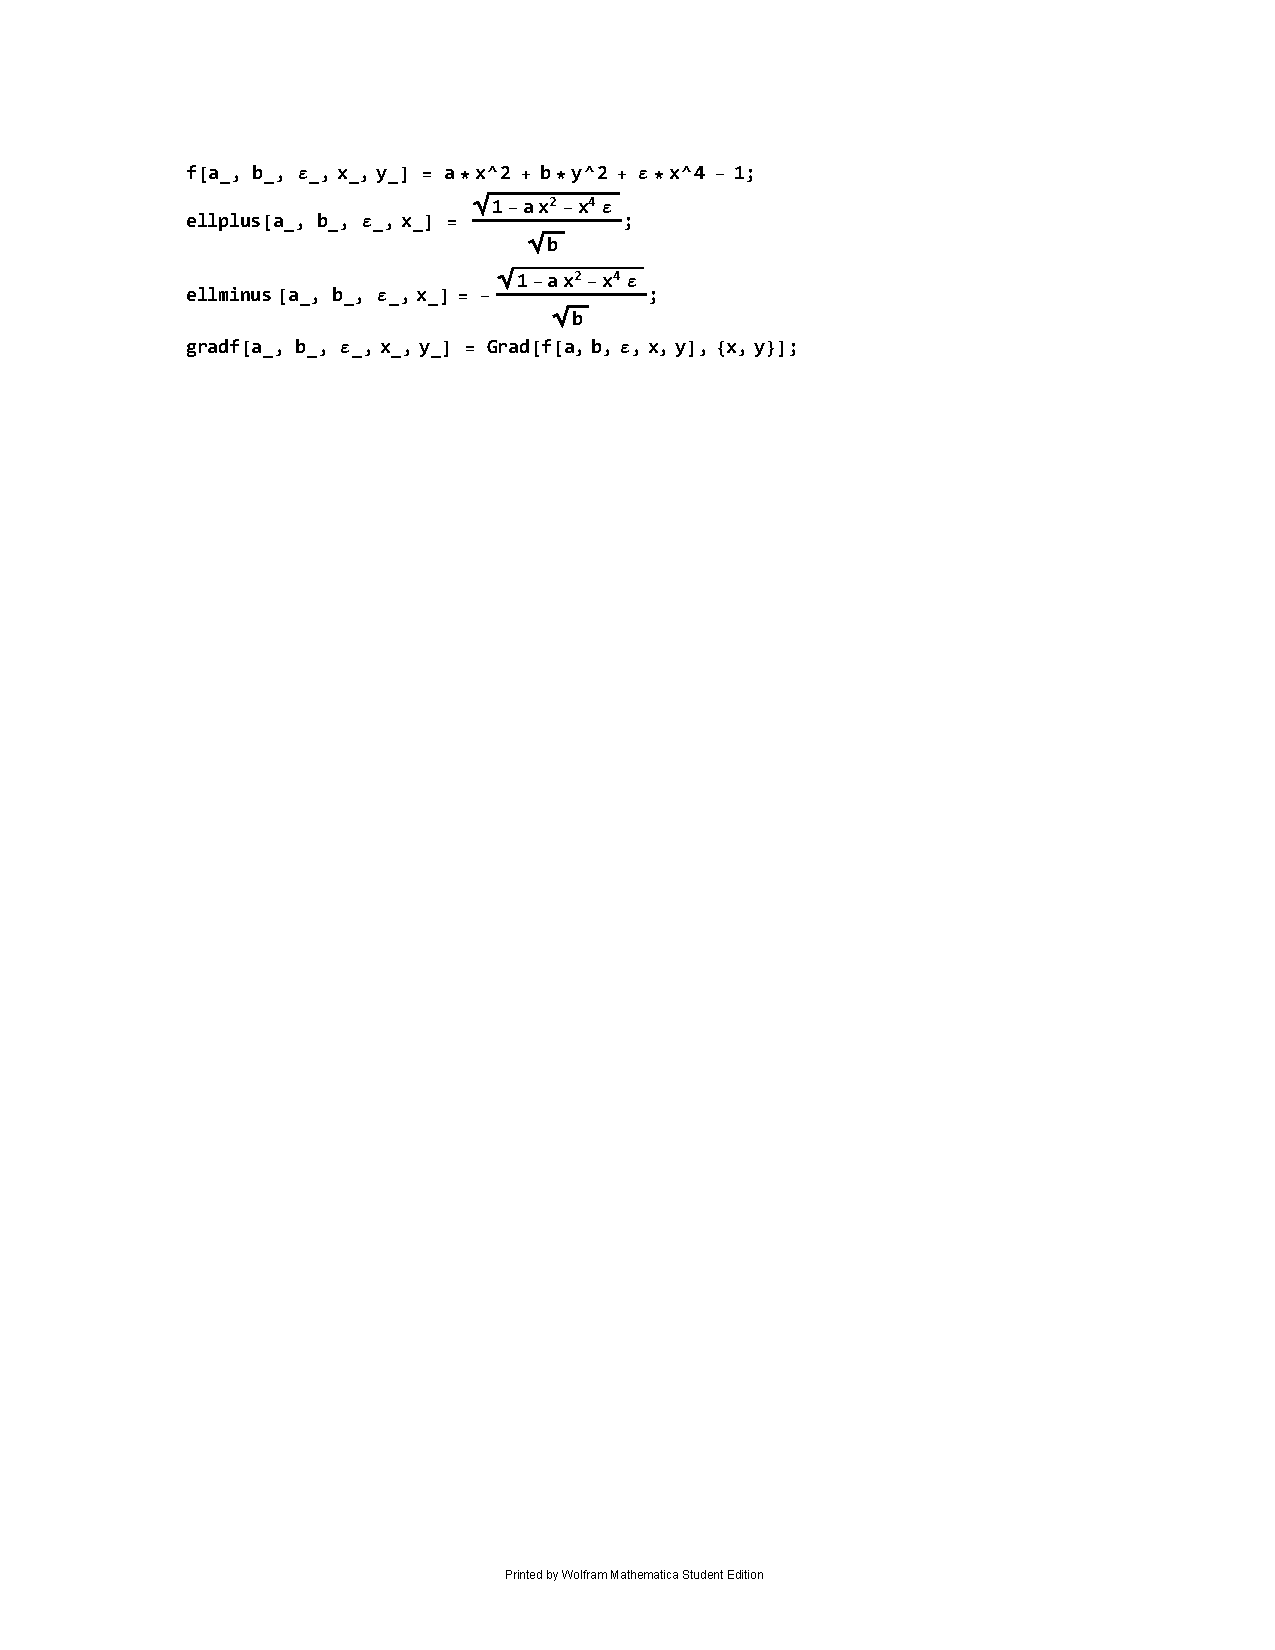
\includepdf[pages={1-4}]{Code.pdf}
\printbibliography


\end{document}
